\documentclass[twocolumn, a4paper,10pt]{article}
\usepackage[utf8]{inputenc}
\usepackage{graphicx}
\usepackage{amsmath}
\usepackage{hyperref}
\usepackage{authblk}
\usepackage{orcidlink}
\usepackage{tikz}
\usetikzlibrary{arrows.meta, shapes.geometric, positioning, calc}
\usepackage{adjustbox}
\usepackage[numbers,sort&compress]{natbib}

%opening
\title{Antenna Array Position Calibration for the Transient Array Radio Telescope}
\author[1]{Timothy C.A. Molteno, \orcidlink{0000-0002-2022-0380}}
\affil[1]{Department of Physics, University of Otago, Box 56, Dunedin, New Zealand}
\affil[1]{Department of Physics \& Electronics, Rhodes University, Makhanda, South Africa}

\begin{document}

\maketitle

\begin{abstract}
The Transient Array Radio Telescope (TART) is an all-sky radio telescope designed to detect transient events. The antenna array contains 24 elements arranged on five spiral arms. For interferometric imaging, the positions of these antennas must be accurately known. This paper presents the technique used to calibrate the antenna positions. The technique is iterative, based on a least-squares minimization that reports outliers which are then re-measured. A method for determining the global orientation of the array using geographical bearings is also presented. This technique is robust, can be performed with simple equipment, and provides accuracy to within 0.01 wavelengths---sufficient for interferometric imaging. Results from the TART deployment at the University of Namibia (UNAM) are presented, demonstrating residual errors at the millimeter scale. The calibration algorithm is implemented in the open-source Python package \texttt{tart-position-cal}~\cite{moltento2026tartpositioncal}.
\end{abstract}

\section{Background and Introduction}

The Transient Array Radio Telescope (TART) is an all-sky imaging interferometer that operates in the L1 band (1.575~GHz). The project is open-source~\cite{tart} and has been deployed widely as a tool to detect radio transients, and also as a platform for the development of new radio imaging algorithms. TART telescopes are often installed as part of a week-long workshop that introduces the attendees to radio astronomy, radio imaging, and interferometry, and at the same time, assembles and installs a TART radio telescope. The position calibration process for the antenna array must determine the relative locations of the antennas to within $\approx 5$~mm in the coordinate system of the phase center of the antenna array.

\begin{figure}
 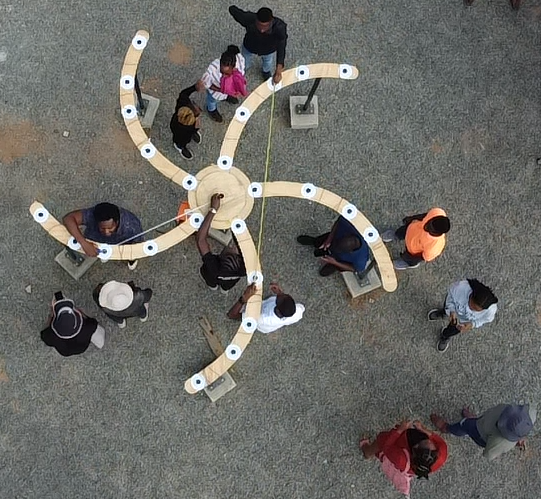
\includegraphics[width=\linewidth]{fig/botswana_calibration.png}
 \caption{Aerial view of a TART being calibrated by attendees at a TART workshop hosted at the Botswana International University of Science and Technology, in March 2025. The atendees are take measurement of the distance between pairs of antennas in order to accurately determine their location.}
\end{figure}

The calibration process must involve easy-to-make measurements, and be robust to accidental errors in measurement. This paper outlines an iterative calibration process that meets these requirements.

\section{Method}

The process involves measuring two kinds of distances. The first are the \emph{radial distances} between the phase-centre and the centre of each antenna. There are $N$ radial distance measurements $r_i$, where $N=24$ is the number of antennas in the array. The second measurements are the pairwise distances between each pair of antennas. There are $\frac{1}{2} N (N-1)$ unique pairs of antennas for an array with $N$ antennas. For the TART there are 276 pairwise distances $\delta_{ij}$ between antennas $i$ and $j$.

As the distance measurements do not constrain the global rotation of the array, an additional constraint is required. It is assumed that the direction between the phase centre and one of the antennas is known. This direction is the measured geographic bearing between one antenna and a distant landmark with known coordinates.

\begin{figure*}
 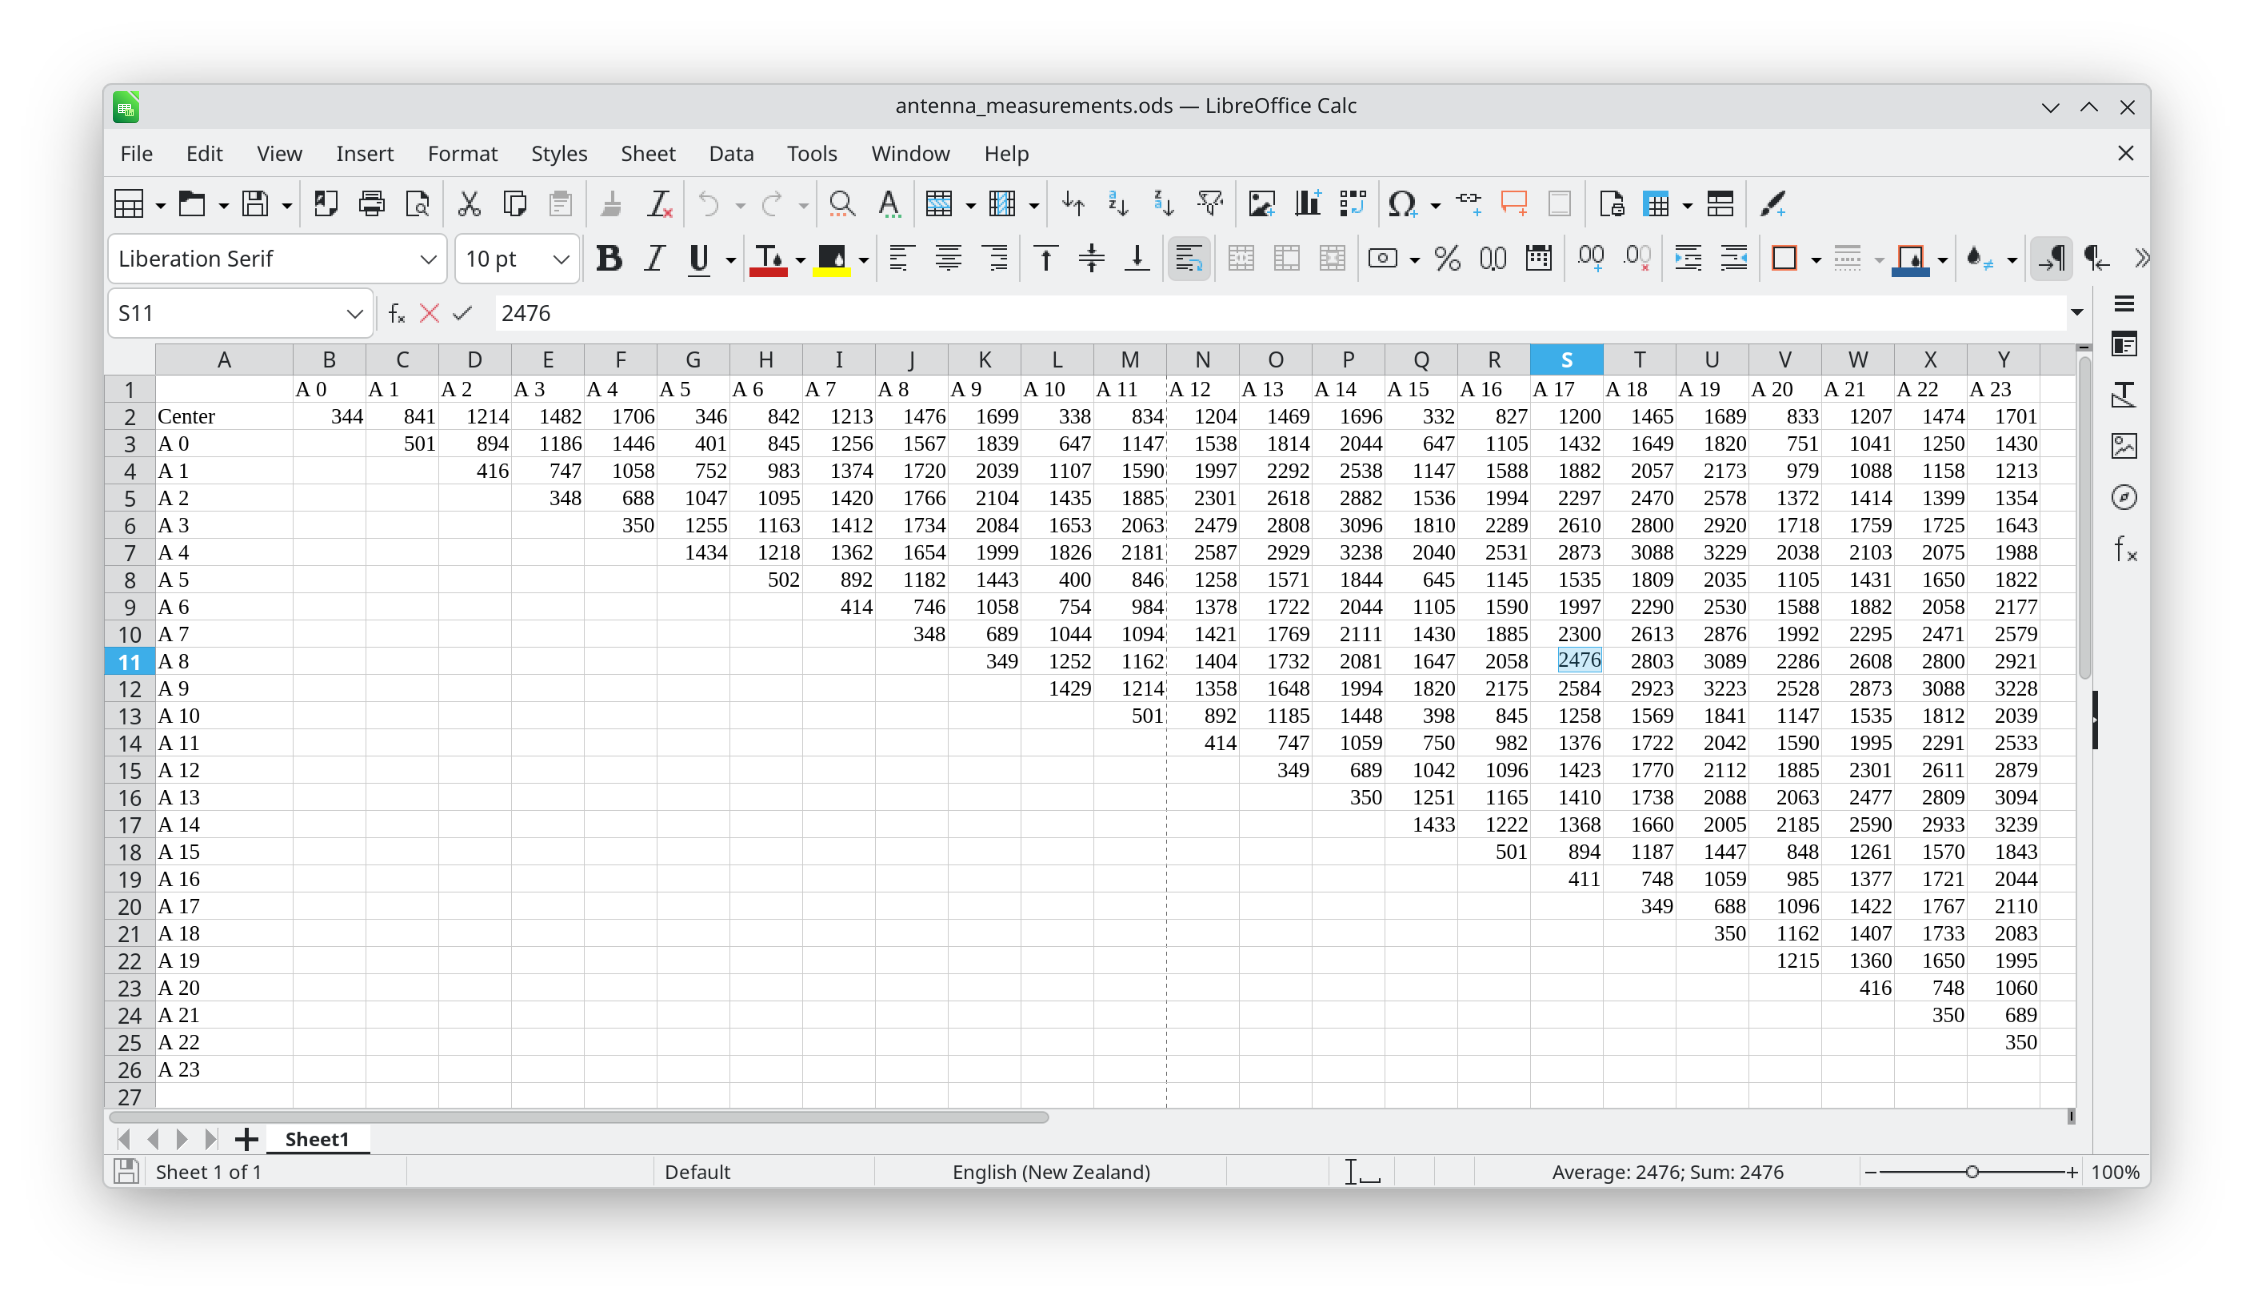
\includegraphics[width=\linewidth]{fig/spreadsheet.png}
 \caption{Spreadsheet with the measurements from a TART antenna array. The highlighted entry shows the distance in mm, between antenna 17, and antenna 8.}
\end{figure*}

The purpose of the algorithm is to estimate the 24 antenna positions in the $x$--$y$ plane that are most consistent with the measurements.

\subsection{Least Squares Estimator}

Given a set $\{x_i, y_i\}$ of 24 antenna positions, and the measurements $r_i$, $\delta_{ij}$, we form a least-squares estimator, $oL(x,y)$:

\begin{align}
 L(x, y) &= L_r(x,y) + L_{ij}(x,y) + \lambda L_\theta(x,y) \\
 L_r(x,y) &= \sum_{i=1}^{N} \left( r_i - \sqrt{x_i^2 + y_i^2} \right)^2 \\
 L_{ij}(x,y) &= \sum_{i,j=1}^{N} \left( \delta_{ij} - \sqrt{(x_i - x_j)^2 + (y_i - y_j)^2} \right)^2 \\
 L_\theta(x,y) &= \left( \theta_k - \arctan\!\left(\frac{x_k}{y_k}\right) \right)^2
\end{align}

where $L_r$ corresponds to the radius measurement residuals, $L_{ij}$ to the pairwise distance residuals, and $L_\theta$ to the global rotation constraint. Here $\theta_k$ is the measured geographic bearing of antenna $k$ relative to the phase centre, and $\lambda$ is a weighting factor (typically $\lambda = 100$) that ensures the rotation constraint is strongly enforced. In practice, the radial residual term is also weighted by a factor of 10 relative to the pairwise term, reflecting the higher confidence in the radial measurements.

\subsection{Algorithm}

The algorithm starts with a set of \emph{initial estimates} of $x_i, y_i$, the coordinates of the $i$th antenna. These are obtained from the telescope's nominal design positions, queried from the telescope API or loaded from a JSON configuration file. From these, the simulated measurements $r^s_i = \sqrt{x_i^2 + y_i^2}$, and $\delta^s_{ij} = \sqrt{(x_i - x_j)^2 + (y_i - y_j)^2}$ are calculated. The least squares estimator $L(x,y)$ is then minimized (as a function of $x_i, y_i$) using the L-BFGS-B algorithm as implemented in the SciPy library~\cite{scipy}, to find the set of antenna positions that produce simulated measurements as close as possible to the actual measurements. The algorithm is implemented in the open-source Python package \texttt{tart-position-cal}~\cite{moltento2026tartpositioncal} and is invoked as:

\begin{verbatim}
tart-position-cal \
    --measurements antenna_measurements.ods \
    --positions antenna_positions.json \
    --output calibrated_antenna_positions.json \
    --rot-index 3 \
    --rot-degrees 18.1125
\end{verbatim}

\begin{figure*}
 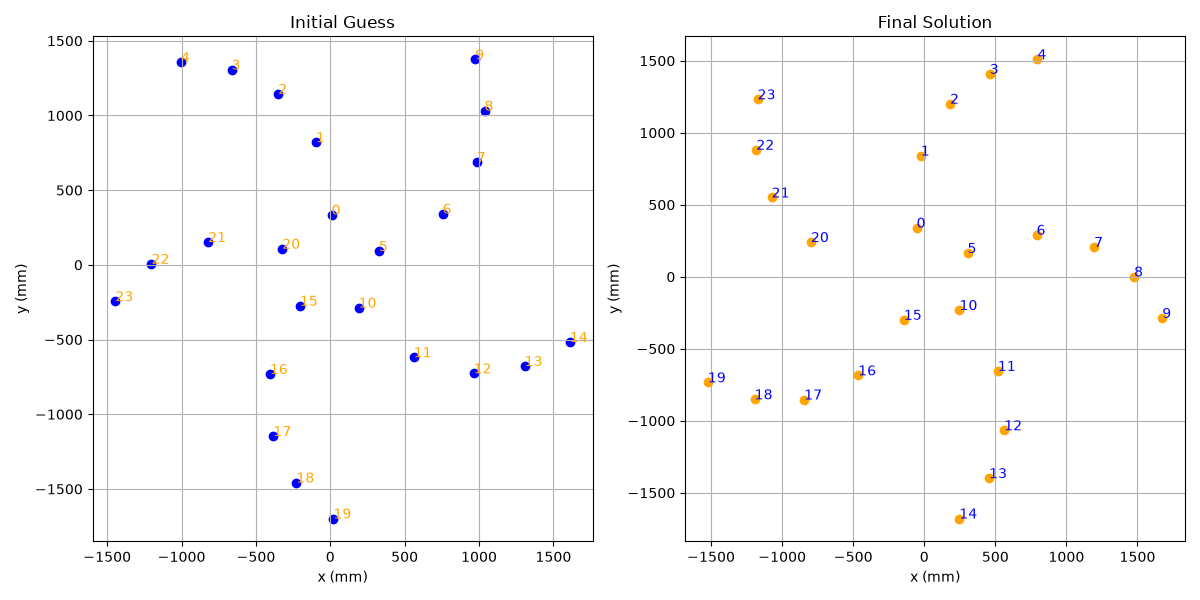
\includegraphics[width=\linewidth]{fig/final_positions.png}
 \caption{Initial position estimates (blue) and the final calibrated positions (orange) for the TART antenna array. Antenna indices are labeled. This shows that the antenna, as constructed was assembled with the spiral arms clockwise oriented, in contrast to the initial position assumptions. }
\end{figure*}

\subsection{Global Orientation Calibration}

The global orientation of the array cannot be determined from distance measurements alone, as the entire array can be rotated about the phase centre without changing any of the $r_i$ or $\delta_{ij}$ values. To fix the absolute orientation, the geographic bearing of one antenna from the phase centre must be measured.

This is accomplished by identifying an antenna arm that aligns with a distant, identifiable landmark visible on satellite imagery (e.g.\ Google Maps). The geographic coordinates (latitude and longitude) of both the telescope site and the landmark are recorded. Using the WGS84 ellipsoid model, the forward azimuth (bearing) from the telescope to the landmark is computed via the inverse geodesic problem as implemented in the PROJ library~\cite{proj}:

\begin{multline}
\beta = \text{atan2}\bigl(\sin\Delta\lambda \cos\phi_2, \\
\cos\phi_1 \sin\phi_2 - \sin\phi_1 \cos\phi_2 \cos\Delta\lambda\bigr)
\end{multline}

where $\phi_1, \lambda_1$ are the telescope coordinates, $\phi_2, \lambda_2$ are the landmark coordinates, and $\Delta\lambda = \lambda_2 - \lambda_1$. This gives the geographic bearing $\beta$ (degrees clockwise from true North).

\begin{figure*}
 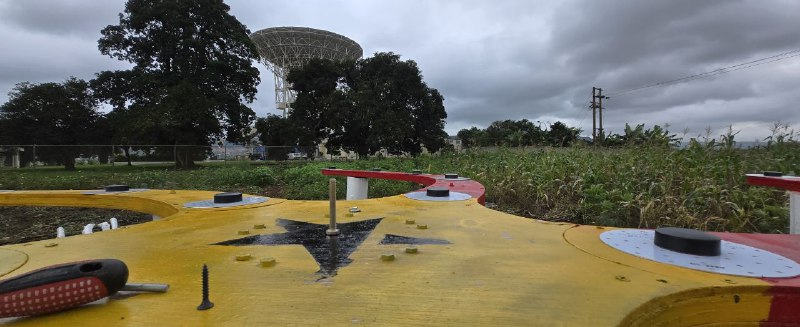
\includegraphics[width=\linewidth]{fig/antenna_9_dish.jpg}
 \caption{At the Ghana TART site, antenna~9 of the TART array aligns approximately with a distant radio telescope dish. This alignment is used to determine the global rotation of the array.}
\end{figure*}

From the array geometry, the expected bearing $\theta_k$ of the reference antenna $k$ is computed from its coordinates in the array's local coordinate system:

\begin{equation}
\theta_k = 90^\circ - \arctan\!\left(\frac{y_k}{x_k}\right)
\end{equation}

The rotation correction $\Delta\theta$ is then:

\begin{equation}
\Delta\theta = -(\theta_k - \beta)
\end{equation}

This rotation is applied to all antenna positions either as a constraint within the least-squares minimization (as $L_\theta$ in Equation~4), or as a post-optimization rotation of the calibrated positions.

\subsection{Residuals and Iterative Refinement}

The differences between the simulated measurements of the calibrated positions and the actual measurements are called residuals. If one or more of the residuals are large, it usually indicates a measurement error. These large residuals are flagged and the corresponding measurements are re-checked and corrected. The optimization is then re-run with the corrected measurements. This iterative process continues until all residuals fall below an acceptable threshold.


\begin{figure}[ht]
\centering
\adjustbox{max width=0.9\linewidth}{%
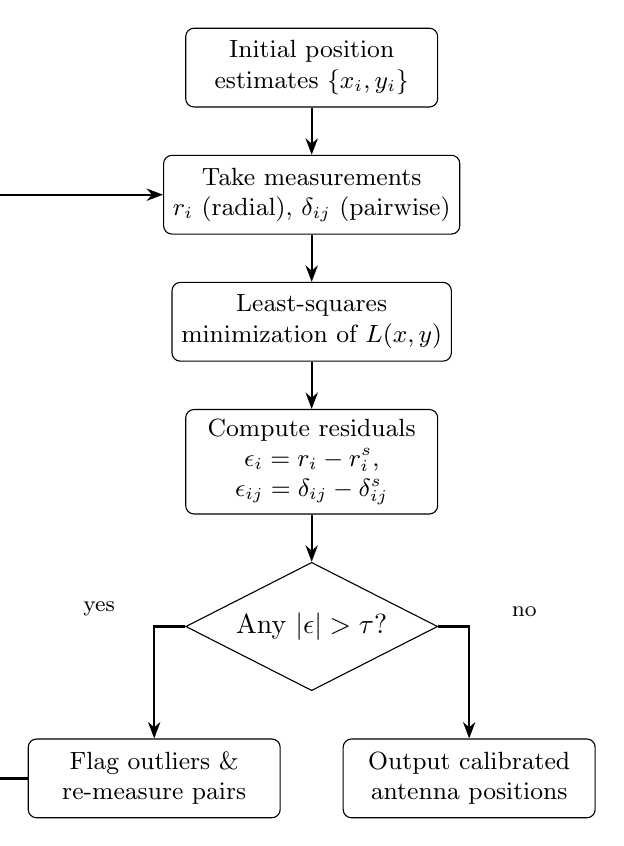
\begin{tikzpicture}[
    node distance=6mm and 4mm,
    box/.style={rectangle, draw, rounded corners=3pt, minimum width=32mm, minimum height=10mm, align=center, font=\small},
    decision/.style={diamond, draw, aspect=1.5, minimum width=32mm, minimum height=10mm, align=center, inner sep=0pt},
    arrow/.style={-{Stealth[scale=0.9]}, thick},
]

\node[box] (start)                    {Initial position\\estimates $\{x_i, y_i\}$};
\node[box] (measure) [below=of start] {Take measurements\\$r_i$ (radial), $\delta_{ij}$ (pairwise)};
\node[box] (optimize) [below=of measure] {Least-squares\\minimization of $L(x,y)$};
\node[box] (residuals) [below=of optimize] {Compute residuals\\$\epsilon_i = r_i - r_i^s$,\\$\epsilon_{ij} = \delta_{ij} - \delta_{ij}^s$};
\node[decision] (check) [below=of residuals] {Any $|\epsilon| > \tau$?};
\node[box] (flag) [below=of check, xshift=-20mm] {Flag outliers \&\\re-measure pairs};
\node[box] (done) [below=of check, xshift=20mm]  {Output calibrated\\antenna positions};

\draw[arrow] (start)    -- (measure);
\draw[arrow] (measure)  -- (optimize);
\draw[arrow] (optimize) -- (residuals);
\draw[arrow] (residuals) -- (check);

\draw[arrow] (check) -| node[above, xshift=-7mm, font=\footnotesize] {yes} (flag);
\draw[arrow] (check) -| node[above, xshift=7mm, font=\footnotesize]  {no}  (done);

\draw[arrow, overlay] (flag.west) -- ++(-5mm,0) |- (measure.west);

\end{tikzpicture}%
}
\caption{Flowchart of the iterative calibration process. Initial position estimates are refined by minimizing the squared residuals against measured radial and pairwise distances. Large residuals (exceeding threshold $\tau$) are flagged for re-measurement, and the optimization is repeated until all residuals are acceptable.}
\label{fig:flowchart}
\end{figure}

\begin{figure}
 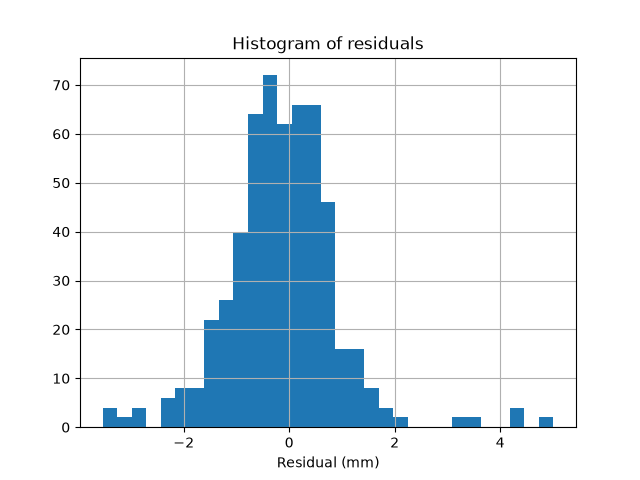
\includegraphics[width=\linewidth]{fig/residual_histogram.png}
 \caption{Histogram of the pairwise distance residuals after calibration, showing that the calibrated positions closely match the measurements. The distribution is centered near zero with a narrow spread.}
\end{figure}

\section{Results: UNAM Deployment}

The TART telescope at the University of Namibia (UNAM) in Windhoek is located at latitude $-22.6121^\circ$, longitude $17.0568^\circ$. The 24 antennas are arranged on five spiral arms, extending to a maximum radius of approximately 1.7~m from the phase centre.

\subsection{Initial Conditions}

The initial position estimates were obtained from the telescope's configuration file, with coordinates in meters converted to millimeters for the optimization. The initial least-squares cost $L(x,y)$ was $6.5 \times 10^7$, indicating substantial disagreement between the nominal positions and the measured distances.

\subsection{Global Orientation}

The global orientation was determined using antenna~3 (index 3 in the array numbering). A distant hill at coordinates $(-22.553822^\circ, 17.077290^\circ)$ was identified as a landmark visible along the antenna arm. The computed bearing from the telescope to the hill was $\beta = 18.1125^\circ$. This angle was used as the rotation constraint $L_\theta$ in the least-squares minimization, with the reference antenna constrained to this bearing.

\subsection{Calibration Results}

The L-BFGS-B optimizer converged after 117 iterations, reducing the cost function from $6.5 \times 10^7$ to $7.66 \times 10^2$. The calibrated antenna positions are given in Table~\ref{tab:positions}. Figure~\ref{fig:unam_differences} shows the displacement of each antenna from its initial position estimate.

\begin{figure}
 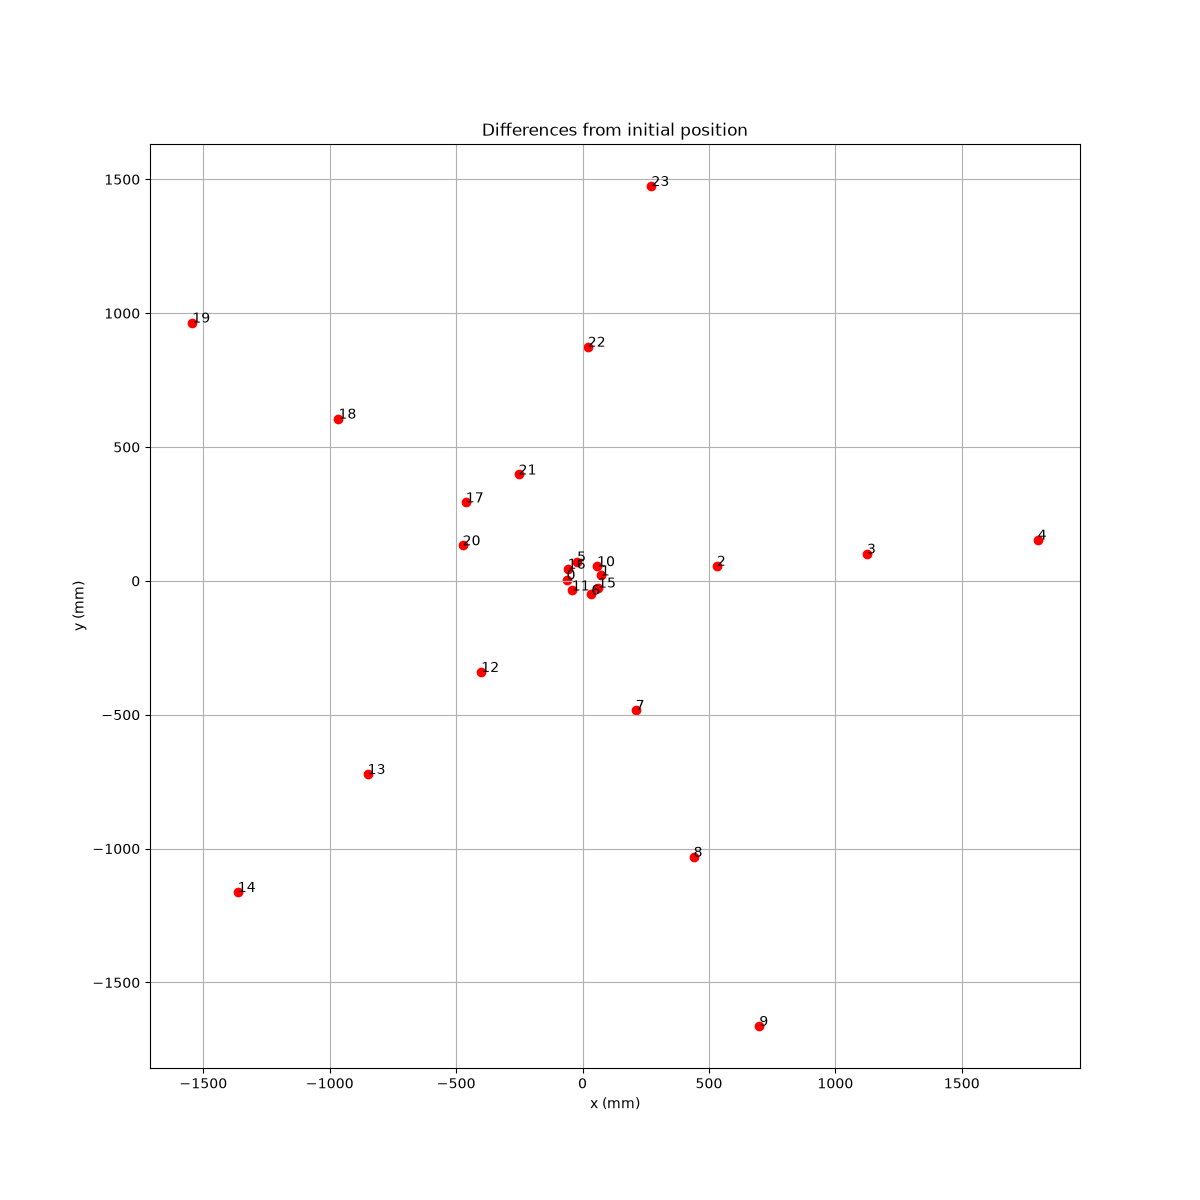
\includegraphics[width=\linewidth]{fig/differences.png}
 \caption{Differences between the initial and final antenna positions for the UNAM array. The vectors show the displacement of each antenna from its nominal position. Antenna indices are labeled.}
 \label{fig:unam_differences}
\end{figure}

\begin{table}[h]
\centering
\caption{Calibrated antenna positions for the UNAM TART array. Coordinates are in meters relative to the phase centre at $[0,0]$.}
\label{tab:positions}
\begin{tabular}{|rrr|}
\hline
Antenna & $x$ (m) & $y$ (m) \\
\hline
 0 & $-0.054$ &  $0.341$ \\
 1 & $-0.025$ &  $0.841$ \\
 2 &  $0.181$ &  $1.202$ \\
 3 &  $0.461$ &  $1.409$ \\
 4 &  $0.796$ &  $1.510$ \\
 5 &  $0.304$ &  $0.164$ \\
 6 &  $0.790$ &  $0.292$ \\
 7 &  $1.195$ &  $0.207$ \\
 8 &  $1.476$ &  $0.002$ \\
 9 &  $1.674$ & $-0.287$ \\
10 &  $0.248$ & $-0.231$ \\
11 &  $0.517$ & $-0.654$ \\
12 &  $0.562$ & $-1.066$ \\
13 &  $0.456$ & $-1.398$ \\
14 &  $0.246$ & $-1.679$ \\
15 & $-0.144$ & $-0.299$ \\
16 & $-0.465$ & $-0.685$ \\
17 & $-0.845$ & $-0.853$ \\
18 & $-1.194$ & $-0.851$ \\
19 & $-1.523$ & $-0.733$ \\
20 & $-0.797$ &  $0.241$ \\
21 & $-1.074$ &  $0.550$ \\
22 & $-1.182$ &  $0.882$ \\
23 & $-1.173$ &  $1.232$ \\
\hline
\end{tabular}
\end{table}

\subsection{Residual Analysis}

The residuals of the pairwise distance measurements after calibration are shown in Figure~\ref{fig:unam_residuals}. The 90th percentile of the absolute residuals is 1.53~mm, indicating that the calibrated positions reproduce the measured distances with sub-millimeter accuracy for the majority of antenna pairs. The largest residuals, listed in Table~\ref{tab:large_residuals}, range up to 5.0~mm and are concentrated in a small number of antenna pairs. These outliers typically indicate measurement errors in the original survey data and would be re-measured in a subsequent iteration of the calibration process.

\begin{figure}
 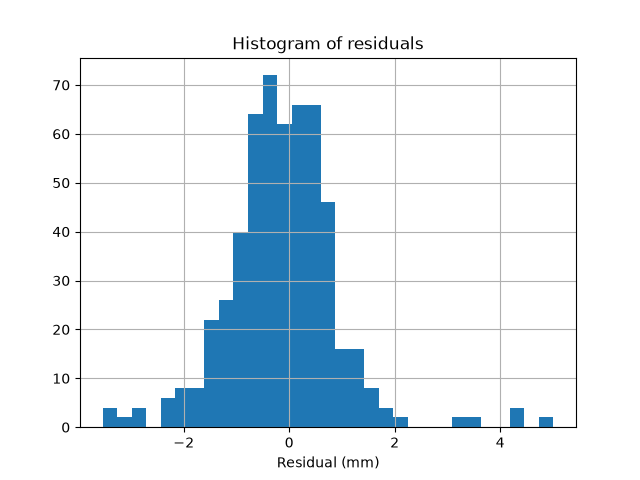
\includegraphics[width=\linewidth]{fig/residual_histogram.png}
 \caption{Histogram of pairwise distance residuals for the UNAM calibration. The 90th percentile is 1.53~mm. The distribution is symmetric around zero with a standard deviation of approximately 1~mm.}
 \label{fig:unam_residuals}
\end{figure}

\begin{table}[h]
\centering
\caption{Largest residuals (exceeding the 90th percentile of 1.53~mm) from the UNAM calibration. Negative residuals indicate that the measured distance was smaller than the calibrated distance.}
\label{tab:large_residuals}
\begin{tabular}{rrr}
\hline
Antenna $i$ & Antenna $j$ & Residual (mm) \\
\hline
19 & 9  & 5.0 \\
17 & 16 & 4.4 \\
 9 & 2  & 4.2 \\
17 & 4  & 3.6 \\
22 & 12 & 3.3 \\
14 & 1  & $-3.2$ \\
17 & 8  & $-2.8$ \\
19 & 4  & $-2.8$ \\
22 & 9  & $-2.3$ \\
 5 & 2  & $-2.2$ \\
14 & 4  & $-2.2$ \\
12 & 3  & $-2.1$ \\
12 & 0  & $-2.0$ \\
14 & 0  & $-2.0$ \\
17 & 9  & $-2.0$ \\
\hline
\end{tabular}
\end{table}

\subsection{Iteratively Reweighted Least Squares}

When survey measurements contain outliers---erroneous distance readings from misaligned tape measures or transcription errors---ordinary least squares can be skewed by those bad measurements. To address this, the \texttt{tart-position-cal} package includes an Iteratively Reweighted Least Squares (IRLS) option, invoked with the \texttt{--irls} flag. IRLS solves a series of weighted least-squares problems, recomputing per-measurement weights after each iteration to down-weight outliers. Two weight functions are available: Tukey's bisquare (default), which zeros out clear outliers entirely, and Huber, which caps the influence of outliers with a saturating linear penalty.

Applying IRLS with Tukey weights to the UNAM data reduced the 90th percentile of absolute pairwise residuals from 1.53~mm to 1.50~mm, while automatically down-weighting the largest outliers without requiring manual re-measurement. The outer loop converged in 10 iterations. Figure~\ref{fig:irls_residuals} shows the residual histogram for the IRLS calibration, which is slightly narrower than the ordinary least-squares result. Compared to the manual iterative re-measurement workflow, IRLS provides a fully automated path to a robust solution, though manual verification of flagged outlier pairs remains advisable for critical deployments.

\begin{figure}
 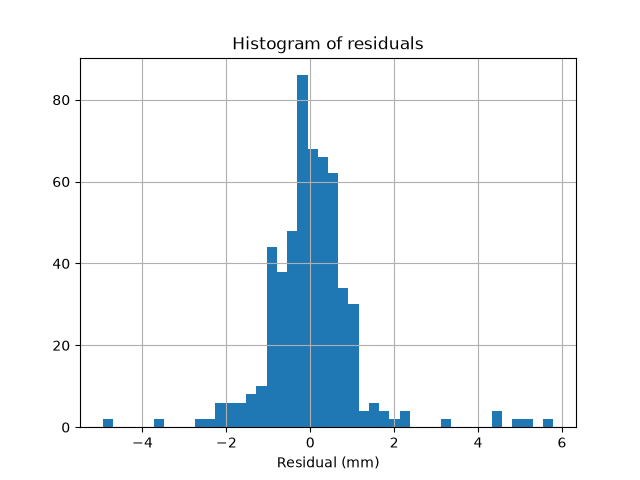
\includegraphics[width=\linewidth]{fig/irls_residual_histogram.png}
 \caption{Histogram of pairwise distance residuals for the UNAM calibration using IRLS with Tukey weights. The 90th percentile is 1.50~mm.}
 \label{fig:irls_residuals}
\end{figure}


\section{Conclusions}

The least-squares position calibration method presented here provides a practical and accurate means of determining antenna positions for the TART radio telescope. The technique requires only a tape measure and a means of recording geographic coordinates for one reference bearing, making it suitable for workshop-based telescope deployments.

Results from the UNAM deployment demonstrate that the method converges reliably from initial position errors on the order of tens of millimeters to a solution with millimeter-scale residuals. The 90th percentile of residuals of 1.53~mm corresponds to approximately $0.008\lambda$ at the L1 frequency, well within the requirement for interferometric imaging.

The iterative nature of the method, with outlier flagging and re-measurement, makes it robust to the inevitable measurement errors that occur during manual surveying. The calibrated positions can be uploaded directly to the telescope API and used for imaging without further adjustment.

\section{Future Work}

The TART telescope operates in the L1 band at 1.575~GHz, which is shared with GNSS signals. The raw telescope data streams contain embedded GNSS satellite signals at known frequencies. Post-processing these signals via software-defined radio techniques could yield direct time-difference-of-arrival (TDOA) measurements between antenna pairs, providing an independent and fully automated means of estimating antenna positions. Since GNSS satellite ephemerides are precisely known, this approach could in principle determine absolute antenna positions without any manual surveying. The main challenge lies in the low signal-to-noise ratio of the GNSS signals in the TART's broad-beam antennas and the short baselines ($<$\,2~m), which produce TDOA values on the order of nanoseconds.

\bibliographystyle{plainnat}
\bibliography{position-cal}

\end{document}
